\section{Competition with two other cells}
\label{geo:section}

Continue with the minimal-active-cell optimal partition from
Lemma~\ref{ext:structure}, satisfying $C>B^2$ and $m\ge5$.
The scalar estimates constrain one cell at a time. We now use the
first-moment identity for the cell with smallest centroid norm to obtain
constraints on pairs of the other centroids.
Relabel the nonzero centroids so that
\[
 r_1\ge r_2\ge\cdots\ge r_m=t>0,
 \qquad
 L=r_1^2+r_2^2,
 \qquad c=r_3^2.
\]
Thus the three largest radii and the chosen smallest radius have distinct
indices, including when some radii are equal.  We will use the centroid
identity for this cell to control the joint distribution of any
two competing scores.

Let $g$ be a standard Gaussian vector in the ambient Euclidean space, and
put
\[
 e=\frac{z_m}{|z_m|},\qquad T=\langle e,g\rangle,
 \qquad
 a_j=-\frac{\langle z_m,z_j\rangle}{|z_m|^2}
 \quad(1\le j<m).
\]
Strict negativity of the off-diagonal products and $\sum_jz_j=0$ imply
\begin{equation}
 a_j>0,\qquad \sum_{j<m}a_j=1.
 \label{geo:coefficients}
\end{equation}
Define the residual vectors and scores by
\[
 w_j=\frac{z_j}{\sqrt C}+a_jte,
 \qquad Y_j=\langle w_j,g\rangle.
\]
Each $w_j$ is orthogonal to $e$.  Consequently $Y=(Y_j)_{j<m}$ is a
centered Gaussian vector independent of the standard normal variable
$T$, and
\begin{equation}
 \frac{\langle z_j,g\rangle}{\sqrt C}=-a_jtT+Y_j.
 \label{geo:decomposition}
\end{equation}
Its covariance matrix $H$ has entries
\begin{equation}
 H_{jk}=\frac{\langle z_j,z_k\rangle}{C}-a_ja_kt^2,
 \qquad h_j:=H_{jj}=r_j^2-a_j^2t^2.
 \label{geo:covariance}
\end{equation}
Since $\sum_{j<m}w_j=0$, every row of $H$ sums to zero; also $H_{jk}<0$
for $j\ne k$.  For distinct $j,k<m$, set
\[
 D_{jk}=\sqrt{h_jh_k-H_{jk}^2}.
\]
These quantities are positive.  Indeed, a linear dependence between
$w_j$ and $w_k$ would give a dependence between $z_j,z_k,z_m$, whereas
every proper subset of the centroids is linearly independent and
$m\ge5$.  In particular, all $h_j$ are positive.

\begin{lemma}[Two competing scores]
\label{geo:pair}
For every pair of distinct indices $j,k<m$,
\begin{equation}
 D_{jk}\le \frac3\pi\,t(1+a_j)(1+a_k).
 \label{geo:pair-bound}
\end{equation}
\end{lemma}

\begin{proof}
Let $K$ be the winning cone for the score $\langle z_m,g\rangle$.
The partition agrees with its score cones almost everywhere, so
$\mathbb E[\mathbf 1_Kg]=z_m$.  The definitions of $T$ and $Y_j$ give
\begin{equation}
 \mathbb E[\mathbf 1_KT]=|z_m|=\sqrt C\,t>Bt,
 \qquad
 \mathbb E[\mathbf 1_KY_j]=\langle w_j,z_m\rangle=0.
 \label{geo:centroid-identities}
\end{equation}
The scores sum to zero.  Their maximum is therefore nonnegative, and
on $K$ we have, by \eqref{geo:decomposition},
\[
 T\ge0,\qquad Y_j\le(1+a_j)tT\quad(j<m).
\]
Fix distinct $j,k<m$ and write
\[
 U=\frac{Y_j}{(1+a_j)t},\qquad
 V=\frac{Y_k}{(1+a_k)t}.
\]
The pair $(U,V)$ is independent of $T$, and its Gaussian density is
bounded above everywhere by
\begin{equation}
 M=\frac{t^2(1+a_j)(1+a_k)}{2\pi D_{jk}}.
 \label{geo:density-bound}
\end{equation}
Here the denominator follows by taking the square root of the
covariance determinant after the two rescalings.

For a real number $x$, write $x_+=\max\{x,0\}$.  Adding the two
zero expectations from \eqref{geo:centroid-identities}, taking a
positive part, and then enlarging the integration region yields
\begin{align*}
 \mathbb E[\mathbf 1_KT]
 &=\mathbb E[\mathbf 1_K(T+U+V)]\\
 &\le\mathbb E\big[
 \mathbf 1_{\{T\ge0,\ U\le T,\ V\le T\}}(T+U+V)_+\big].
\end{align*}
For a fixed $s\ge0$, within $u\le s$, $v\le s$ the positive integrand
is supported on the triangle with vertices $(s,s)$, $(s,-2s)$, and
$(-2s,s)$. The corresponding unweighted planar integral is
\begin{align*}
 \int_{u\le s}\int_{v\le s}(s+u+v)_+\,dv\,du
 &=\int_0^\infty\int_0^\infty(3s-a-b)_+\,db\,da\\
 &=\int_0^{3s}\int_0^{3s-a}(3s-a-b)\,db\,da
 =\frac{(3s)^3}{6},
\end{align*}
where $a=s-u$ and $b=s-v$. Figure~\ref{fig:residual-score-triangle}
shows this integration region and its affine integrand.
\begin{figure}[htbp]
  \centering
  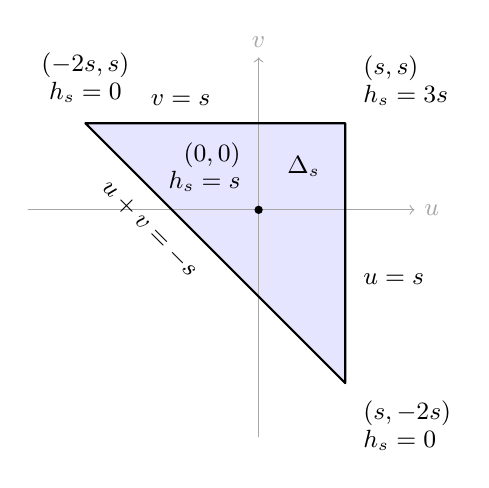
\begin{tikzpicture}[x=1.10cm,y=1.10cm,line cap=round,line join=round,
                      font=\small]
    \fill[blue!10] (-2,1) -- (1,1) -- (1,-2) -- cycle;
    \draw[gray!70,->] (-2.66,0) -- (1.80,0) node[right] {$u$};
    \draw[gray!70,->] (0,-2.62) -- (0,1.76) node[above] {$v$};
    \draw[thick] (-2,1) -- (1,1) -- (1,-2) -- cycle;
    \node[above=4pt,align=center] at (-2,1)
      {$(-2s,s)$\\[-1pt] $h_s=0$};
    \node[above right=3pt,align=left] at (1,1)
      {$(s,s)$\\[-1pt] $h_s=3s$};
    \node[below right=3pt,align=left] at (1,-2)
      {$(s,-2s)$\\[-1pt] $h_s=0$};
    \node[above=3pt] at (-.90,1) {$v=s$};
    \node[right=3pt] at (1,-.80) {$u=s$};
    \node[rotate=-45,below=4pt] at (-1.02,.02) {$u+v=-s$};
    \node at (.52,.50) {$\Delta_s$};
    \fill (0,0) circle[radius=1.5pt];
    \node[above left=3pt,align=right] at (0,0)
      {$(0,0)$\\[-1pt] $h_s=s$};
  \end{tikzpicture}
  \[
    \int_{\Delta_s}h_s(u,v)\,du\,dv
    =\underbrace{\frac{(3s)^2}{2}}_{\text{area}}
      \underbrace{\frac{3s+0+0}{3}}_{\text{mean affine height}}
    =\frac{27s^3}{6}.
  \]
  \caption{For fixed $T=s>0$, the positive integrand is supported,
  within $u\le s$ and $v\le s$, on
  $\Delta_s=\{(u,v):u\le s,\ v\le s,\ s+u+v\ge0\}$.
  Here $h_s(u,v)=s+u+v$ is an affine height, with the displayed values at
  the vertices and barycenter. The shading marks the integration region,
  not the support or density of the Gaussian pair $(U,V)$.
  Multiplying the unweighted integral by the density bound $M$ gives
  the estimate used in the proof. At $s=0$ the triangle degenerates and
  the integral is zero.}
  \label{fig:residual-score-triangle}
\end{figure}

Using \eqref{geo:density-bound},
independence, and $\mathbb E[T_+^3]=2/\sqrt{2\pi}$, we obtain
\[
 Bt<\mathbb E[\mathbf 1_KT]
 \le \frac{27M}{6}\,\mathbb E[T_+^3]
 =\frac{9t^2(1+a_j)(1+a_k)}{2\pi\sqrt{2\pi}\,D_{jk}}.
\]
Since $B=3/(2\sqrt{2\pi})$, this gives
\eqref{geo:pair-bound}, in fact with a strict inequality.
\end{proof}

The pairwise inequality becomes useful for the partition problem when
we sum it over competitors with the largest centroid lengths. The
negative off-diagonal covariances prevent all of these pairwise
determinants from being small simultaneously.

\begin{corollary}[Constraints on the three largest radii]
\label{geo:constraints}
The quantities $L,c,t$ satisfy
\begin{align}
 (c-t^2)(L-c-2t^2)
 &\le8\left(\frac3\pi\right)^2t^2,
 \label{geo:first-constraint}\\
 \frac32(c-t^2)^2
 &\le10\left(\frac3\pi\right)^2t^2.
 \label{geo:second-constraint}
\end{align}
\end{corollary}

\begin{proof}
For the first inequality, the signs and row sums of $H$ give
\[
 H_{31}^2+H_{32}^2
 \le (|H_{31}|+|H_{32}|)^2\le h_3^2.
\]
It follows that
\begin{equation}
 D_{31}^2+D_{32}^2\ge h_3(h_1+h_2-h_3).
 \label{geo:row-lower}
\end{equation}
By \eqref{geo:covariance} and $0<a_j\le1$,
\[
 h_3\ge c-t^2\ge0,
 \qquad h_1+h_2-h_3\ge L-c-2t^2.
\]
If $L-c-2t^2\ge0$, these inequalities and \eqref{geo:row-lower}
show that
\[
 D_{31}^2+D_{32}^2\ge(c-t^2)(L-c-2t^2).
\]
If $L-c-2t^2<0$, the same conclusion follows from the
nonnegativity of the determinant squares.

On the other hand, Lemma~\ref{geo:pair} gives
\[
 D_{31}^2+D_{32}^2
 \le\left(\frac3\pi\right)^2t^2
 (1+a_3)^2\big((1+a_1)^2+(1+a_2)^2\big).
\]
Because $a_1+a_2\le1-a_3$,
\[
 (1+a_1)^2+(1+a_2)^2
 \le (2-a_3)^2+1.
\]
For $0\le x\le1$, the identity
\[
 8-(1+x)^2\big((2-x)^2+1\big)=(1-x)^2(3-x^2)\ge0
\]
therefore proves \eqref{geo:first-constraint}.

For the second inequality, let
$\rho_{jk}=H_{jk}/\sqrt{h_jh_k}$ for $1\le j<k\le3$.
These correlations belong to $[-1,0]$.  Since
\[
 0\le\operatorname{Var}\left(\sum_{j=1}^3\frac{Y_j}{\sqrt{h_j}}\right)
 =3+2\sum_{1\le j<k\le3}\rho_{jk},
\]
we have
\[
 \sum_{j<k\le3}\rho_{jk}^2
 \le\sum_{j<k\le3}|\rho_{jk}|\le\frac32.
\]
Each $h_j\ge c-t^2\ge0$ for $j\le3$.  Thus
\begin{equation}
 \sum_{j<k\le3}D_{jk}^2
 =\sum_{j<k\le3}h_jh_k(1-\rho_{jk}^2)
 \ge\frac32(c-t^2)^2.
 \label{geo:correlation-lower}
\end{equation}
To bound the sum furnished by Lemma~\ref{geo:pair}, put
\[
 s_1=a_1+a_2+a_3,\qquad
 s_2=a_1a_2+a_1a_3+a_2a_3,\qquad s_3=a_1a_2a_3.
\]
Equation~\eqref{geo:coefficients} implies
$0\le s_1\le1$, $0\le s_2\le s_1^2/3\le1/3$, and $s_3\ge0$.
Expanding in these elementary symmetric functions gives
\begin{align*}
 \sum_{j<k\le3}(1+a_j)^2(1+a_k)^2
 &=3+4s_1+2s_1^2+2s_1s_2+s_2^2-(6+2s_1)s_3\\
 &\le3+4+2+\frac23+\frac19=\frac{88}{9}<10.
\end{align*}
Squaring \eqref{geo:pair-bound}, summing over the three pairs, and
combining with \eqref{geo:correlation-lower} proves
\eqref{geo:second-constraint}.
\end{proof}
